\section{Introduction}
\label{sec:intro}

Large language model (LLM) agents increasingly act through the Model
Context Protocol (MCP), a fast-growing standard that exposes external tools
(file stores, databases, web services, developer platforms) behind a uniform
calling interface. As agents move into production, the practical question is
no longer whether a model can call a tool, but whether it accomplishes the
user's goal across many real, interacting services. Existing benchmarks mostly
score one of two proxies: the final natural-language answer, matched to a
reference string, or the set of tools the agent was expected to call. Both are
fragile where deployment matters. Reference answers go stale when they depend
on live data, and fixed tool lists are not recoverable from the prompt alone,
so they can penalize different but equally valid routes.

\begin{figure*}[t]
  \centering
  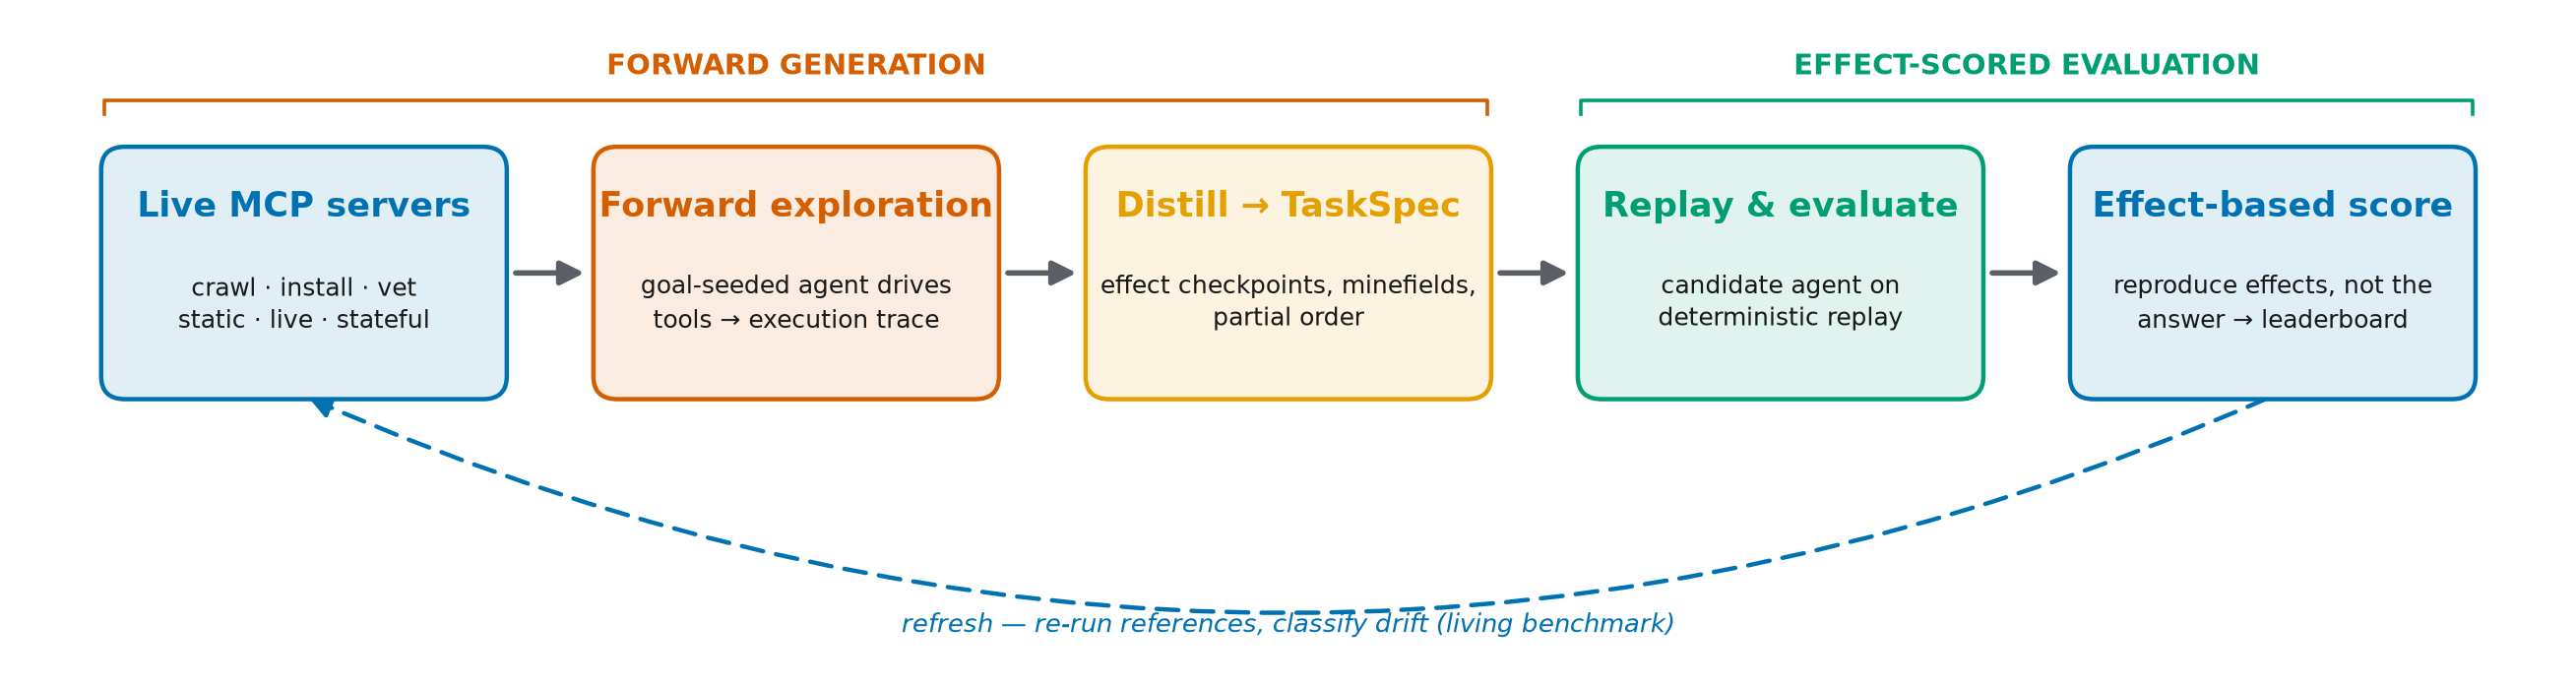
\includegraphics[width=\textwidth]{figures/fig_pipeline.png}
  \caption{The DynamicMCPBench pipeline. \textbf{Forward generation:} a
    goal-seeded agent explores live MCP servers, and each successful execution
    trace is distilled into a path-agnostic \emph{TaskSpec}: effect
    checkpoints, minefields, and a partial order. \textbf{Effect-scored
    evaluation:} a candidate agent runs on deterministic replay and is graded
    only on whether it reproduces those effects, with any effect-equivalent
    tool and never on its final answer. A periodic \emph{refresh} re-runs
    references and classifies drift, keeping the benchmark live.}
  \label{fig:pipeline}
\end{figure*}

We argue that the organizing object of the benchmark should be neither the
answer nor the tool list, but the \emph{execution trace}. \textbf{DynamicMCPBench}
is a framework rather than a fixed dataset: a practitioner can run it on their
own MCP servers, or let it collect servers automatically to measure general
agentic ability. Given servers and candidate models, it (i)~generates realistic
goals from tool surfaces; (ii)~drives an explorer agent to solve each goal
\emph{live}, recording successful trajectories; (iii)~distills each trajectory
into path-agnostic \emph{effect checkpoints}, forbidden-action
\emph{minefields}, and a partial order; and (iv)~scores a candidate only on
whether its trajectory reproduces those effects, with any effect-equivalent
tool, never on its final answer (Figure~\ref{fig:pipeline}). Because every
required tool was actually used to reach the goal, spurious ``unnecessary
tool'' labels cannot arise by construction.

For industrial deployments, this makes benchmarking a deployment-specific
diagnostic. A company can run the pipeline on its private MCP server fleet,
generate tasks reflecting its workflows, and compare agents under the same
effect-scored protocol used in our public study. The public benchmark serves
as a calibrated reference point: failures can be attributed not only to the
model, but also to task length, cross-server composition, or properties of the
company's tools.

To demonstrate the framework and chart where current agents stand, we run it
over 121 live MCP servers, generating 750 tasks evenly spread across 15 task
categories. The categories cover distinct tool-use challenges, from single-tool
requests to long cross-server chains and look-alike-tool confusions. We evaluate
24 API-served and locally hosted models. Even the strongest agents solve only
about half of the tasks under pass$^3$ (all three independent attempts must
succeed), 31\% of tasks are solved by no model, and accuracy falls steadily as
the required tool chain lengthens. A human validation study confirms that the
automatic, answer-agnostic scoring is reliable.

The contributions are: (i)~a \emph{reusable framework} that turns live MCP
servers and models into a trace-grounded benchmark, with deployment-specific
failure breakdowns (\S\ref{sec:benchmark}); (ii)~an \emph{answer-agnostic,
effect-based} scorer that credits any trajectory reproducing the required
effects and is validated against human judgment
(\S\ref{sec:benchmark},~\S\ref{sec:results}); (iii)~a large demonstration
study (24 models, 121 servers, 750 tasks) showing that current agents struggle
with long, multi-step tasks, stratified by task length and category
(\S\ref{sec:results}); and (iv)~a public, anonymized release of both the
framework and generated benchmark.
